\chapter{The Use Case of Bayesian Inference in Hydrological Model}

In this chapter, we focus on the hydrological model that is used in this thesis. An overview will be given, followed by the explanations of hyperparameters. In the last section, the dataset used in this thesis is observed and visualized to provide a practical understanding for the hydrological model.


\section{Overview of the Hydrological Model}
The HBV-SASK conceptual model is a renowned mathematical model that is commonly used in the field of hydrology. HBV is a model that describes the subroutines for snow accumulation and melts, for soil moisture accounting and river routing~\cite{hbv}. SASK stands for the province of Saskatchewan, the province in Canada in which the model is developed. The creation of the HBV-SASK model is therefore based on the HBV model but involves local data calibration and integration with local water management needs~\cite{sask}.

The HBV-SASK model has twelve different hyperparameters, of which seven are relevant to this thesis~\cite{ivana_relevant_params}. These include~\cite{hydrology}:

\begin{itemize}
  \item TT: Ranges from -4 to 4. It stands for the air temperature threshold in °C for melting/freezing and separating rain and snow.
  \item C0: Ranges from 0 to 10. It describes the base melt factor in mm/°C per day.
  \item $\beta$ (beta): Ranges from 0 to 3. It depicts the shape parameter (exponent) for the soil release equation.
  \item ETF: Ranges from 0 to 1. It describes the temperature anomaly correction in 1/°C of potential evapotranspiration.
  \item FC: Ranges from 50 to 500. It depicts the field capacity of soil in mm.
  \item FRAC: Ranges from 0.1 to 0.9. It stands for the fraction of soil release entering the fast reservoir.
  \item K2: The slow reservoir coefficient ranges from 0 to 0.05, which determines what proportion of the storage is released per day.
\end{itemize}

To run this model, these hyperparameters need to be determined. Since the only prior information given is the lowest and the highest bound of each hyperparameter, uncertainty quantification of these hyperparameters is, therefore, necessary to gain posterior information. Apart from these hyperparameters, the starting and the end date of the period that is used for uncertainty quantification are also required to be specified~\cite{hydrology}. However, the very first phase at the start is used for the spin-up phase, in which the model runs for some time using historical data. This phase stabilizes internal model states such as soil moisture and groundwater levels, which are important for accurate simulation~\cite{hydrology}.

\section{Overview of the Data Set}
There are two existing data sets to the hydrological model, which are respectively called Oldman Basin and Banff Basin, since they are each measured at the Oldman River and in the town of Banff in Alberta, Canada~\cite{hydrology_dataset}. The value that is measured is called streamflow. It describes the movement of water within a river or stream channel and is the combined result of all climatological and geographical factors that operate in a drainage basin~\cite{streamflow}. Both of these data sets are presented in the format of a time series, in which the value of each measurement is collected against the dates over a long period. The Oldman basin data set is available from 1979 to 2008, whereas the Banff basin data set is available from 1950 to 2011~\cite{hydrology}.

Since the data is presented in a format of time series, a time series decomposition is required to present more information on trends, and seasonal and regression effects~\cite{time_series}. After the decomposition, the trend, seasonal, and residue of the dataset over the whole period can be observed. For the time series decomposition in this section, the function TSA.seasonal.seasonal\_decompose from the python framework stats models is used~\cite{stat_models_decompose}.

First, we take a look at the result of the decomposition of the Oldman basin data set. It is shown in Figure 3.1. The seasonal component of this time series is regular over the years. However, there were significant peaks around the early 1980s, mid-1990s, and around 2005. The streamflow in these periods is higher than anytime else, which indicates that there might be possible heavy rainfalls, floods~\cite{hydrology}, or even ecologic disasters. Anomalies in this period can be also found in the residue component, which confirms that there might be odd behaviors happening in these periods. Therefore, quantifying the uncertainty of these three periods would be a challenging task.

\begin{figure}
    \centering
    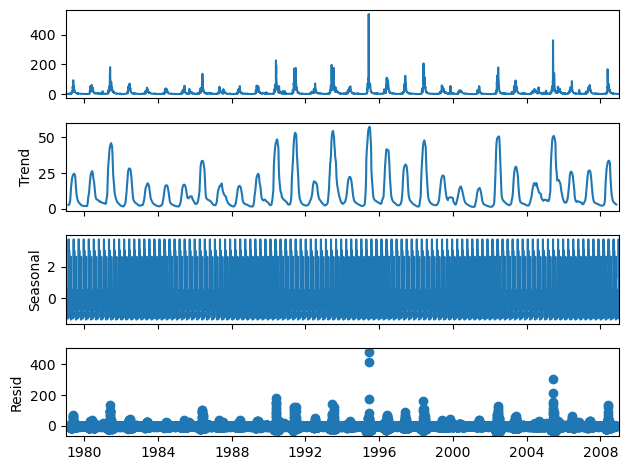
\includegraphics[width=0.8\textwidth]{figures/dataset_time_series/Oldman.png}
    \captionsetup{width=.8\textwidth}
    \caption{Time series decomposition of the Oldman dataset}
    \label{fig:enter-label}
\end{figure}


We then take a look at the result of the decomposition of the Banff basin data set. It is shown in Figure 3.2. Similar to the case of Oldman Basin, it shows a regular seasonal component. The trend, on the other hand, fluctuates across the entire measured period but does not show a general upward or downward direction. This means, that the whole measurement is indeed relatively stable. However, the fluctuation might still impose an influence on the accuracy and stability of uncertainty quantification. The residuals of the Banff basin data set are much more varied than the Oldman basin data set. There are obvious clusters of high activity and anomalies, which confirms that the uncertainty quantification of this data set might be a hard task to deal with.

\begin{figure}
    \centering
    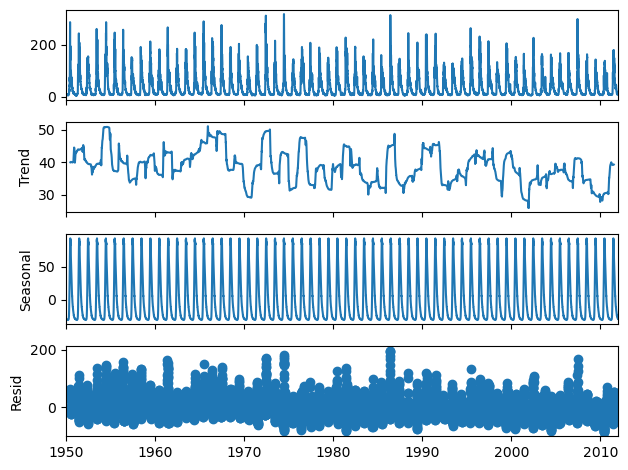
\includegraphics[width=0.8\textwidth]{figures/dataset_time_series/Banff.png}
    \captionsetup{width=.8\textwidth}
    \caption{Time series decomposition of the Banff dataset}
    \label{fig:enter-label}
\end{figure}

\section{Task}
Since the task of this paper is to caliber the input algorithm parameters of the hydrology model, the ultimate goal is to acquire the posterior of the parameters. The main idea in this use case is that we infer the posterior probability of each parameter using Markov chain Monte Carlo. The exact process goes as follows: First, a model is created with the configuration of the period and target distributions being given. Then, we select an appropriate Markov chain Monte Carlo algorithm and perform sampling to solve the Bayesian inference. In this process, the output of each generated set of parameter arrays will be calculated by the model. The output will be later compared to the measured data points, which will provide the algorithm with an acceptance rate. In each iteration, the algorithm decides whether to accept or reject this sample. After all these iterations, the posterior probability is obtained and is prepared to be used on a testing data. Last but not least, we compare the projected results that are calculated by the model to the measured result. Since the posterior probability that is obtained is denoted in the form of a list of sampled data, we can use the Monte Carlo simulation to generate a certain amount of samples, pass them into the model and acquire the result. Then, we can either calculate the mean of the results or sample the maximum of the result to compare them with the actual data.

In order to operate the training and the testing data periods are needed to be determined and extracted. For the Oldman Basin, the trend of the data from 1990 until 2000 remains constantly fluctuated within a specific upper bound and a specific lower bound, which indicates the stability of the record. Therefore, the posterior is inferred by the time period of the entire 90s. An additional ten years beforehand, which is equivalent to the time period on which the posterior is trained, is used for the spin up phase. The time period after 2000 is then used as the testing phase. Since there are some anomalies around 2005, any time period that includes the year 2005 would be an excellent time period for testing. For the Banff Basin data set, the recorded data is kept constant after the year 1970 and the year 1990. However, in order to use the data in the 2000s for testing purpose, the data before 1990s does not play such an important role. Therefore, we use the data in the time period of the 1990s for training purpose, whereas the 10 years beforehand are used for the spin up phase. The entire time period after the 2000s would be excellent for testing purpose, since anomalies and extreme values can be found throughout the entire sequence.

To test the generalized application of the algorithm, we select three challenging yet representative periods for testing, with one being long (5 years), another being medium long (around 2 years) and the other being short (1 year). Due to the constant fluctuation of the Banff basin data set, we could select a long period within it to perform uncertainty quantification. Since the residue in the early 1970s seems to show extreme anomalies, we select 1970 to 1974. The other two periods are both picked from the Oldman Basin data set. The period from 1994 to 1996 is chosen, since there are apparent anomalies of the residue in this period. Another period is the year 2005, since there are also anomalies being showcased in this year.
